\section{Background}
\subsection{A Closer Look At The Problem}
To get a better understanding of the problem Optika is trying to solve, it is
best to look at an example of said problem. Currently, the program Tramonto has
a massive input file filled with complex, non-intuitive inputs. Figure
\ref{tramontoInputFigure} is just small section of this input file.
\begin{figure}
  \centering
  {\footnotesize
  \begin{verbatim}
************* DIMENSION PARAMETERS ********************************************
@ -1. -1. -1. -1. 10. 	Length_ref Density_ref Temp Dielec_ref VEXT_MAX 
************* MESH PARAMETERS *************************************************
@ 3 	Ndim 
@ 3. 2. 2. 	Size_x(idim): idim=0,Ndim-1 
@ 0.25 0.25 0.25 	Esize_x(idim): idim=0,Ndim-1 
@ -1 2 	Type_bc(x0,: left, right) (-1=IN_WALL, 0=IN_BULK, 1=PERIODIC, 2=REFLECT, 3=LAST_NODE) 
@ 1 1 	Type_bc(x1,: down, up) 
@ 1 1 	Type_bc(x2,: back, front) 
  \end{verbatim}
  }
  \caption[Tramonto Input]{An example of the complex input file used by Tramonto}
  \label{tramontoInputFigure}
\end{figure}
This input file is hard to read and non-intutive, not to mention it could 
easily intimidate
a new user. In fact, Tramonto's current input system is so complicated, 
that it is recommended most users simply take sample input files and just 
modify them for their needs.

\subsection{Why Not Something Else?}
Instead of relying on current solutions GUI solutions to solve the above problem, Optika was created in order to address
a number of constraints.
\subsubsection{Something Simple}
Current GUI frameworks like Qt (on which Optika is based), GTK+, and Cocao are incredibly roboust. But
because of this they are also large and complicated. When looking for a solution to the 
scientific application interface problem, we need something that is simple. Otherwise, as mentioned
above, developers will be hesistent to use it.

\subsubsection{Cross-Platform}
Having a better user interface can lead to having a wider user base. When adding the functionality
of a GUI to your application, you don't want to accidentally exclude some of your users by
using a technology that won't work on their platform of choice. Cocao for example only works on
Mac OSX systems. By using Qt as it's underpinnings, Optika is able to work on a wide variety of
platforms.

\subsubsection{Trilinos Integration}
Optika was developed as part of the Trilinos project. Trilinos is a set of C++ libraries
used extensively throughout the scientific community. Since Optika is part of Trilinos,
we wanted it to have tight integration with constucts that were already in place inside
of Trilinos. By creating our own GUI solution, Optika allows users already familiar
with the Trilinos framework to take advantage of the capabilities Optika has to offer.

\section{Optika Overview}
\subsection{GUI Fundamentals}
An Optika based GUI is laid out in a hirerachical fashinon as shown in Figure \ref{paramlistFigure}.
This hierachy is made up of Parameters and ParameterLists. Parameters can simply be thought of as single input for
a program. A ParameterList is simply a collection of Parametes and other ParameterLists. When a ParameterList
is part of another ParameterList we call it a sublist. Optika then uses these ParameterLists to dynamically
generate a GUI which is used to obtain input from the user.
		\begin{figure}
			\centering
			\begin{picture}(50,150)(0,0)
				\put(10,0){\line(0,1){145}}
				\put(0,150){${Parameter List}$}
				\put(10,130){\line(1,0){15}}
				\put(28,127){$Parameter$}
				\put(10,110){\line(1,0){15}}
				\put(28,107){$Parameter$}
				\put(10,90){\line(1,0){15}}
				\put(28,87){$Parameter$}
				\put(10,70){\line(1,0){15}}
				\put(28,67){$Parameter List$}
				\put(38,0){\line(0,1){62}}
				\put(38,47){\line(1,0){15}}
				\put(56,44){$Parameter$}
				\put(38,22){\line(1,0){15}}
				\put(56,24){$Parameter$}
			\end{picture}
			\caption[GUI Layout]{The hierarchical layout of the GUI}
			\label{paramlistFigure}
		\end{figure}
Parameters in Optika are typed. Parameters can be any one of the following types:
  \begin{multicols}{2}
		\begin{itemize}
			\item int
			\item short
			\item float
			\item double
			\item string
			\item boolean
			\item arrays of int, short, double, and string
		\end{itemize}
	\end{multicols}

When editing a parameter in Optika different ``widgets'' are used to change the parameters value. A widget is simply
a graphical construct used for obtaining input from the user. For number types, a spin box (Figure~\ref{spinboxfig}) is used to obtain input. 
If the valid values for a string type were specified (something that will be discussed later), a combo box (Figure~\ref{comboboxfig}) is used.
Otherwise a line edit (Figure~\ref{lineeditfig}) is used to edit a string parameters. For booleans, a combo box (Figure~\ref{comboboxfig}) 
is also be used. For arrays, a pop-up box containing numerous input widgets is used. The widget type is determined by the
array type (e.g. for numerical types a series of spinboxes would be used, for string types comboxes or lineedits are used, etc.). 
	\begin{figure}
		\centering
		\subfigure[A Spin Box]{
			\label{spinboxfig}
			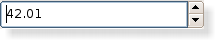
\includegraphics[scale=0.5]{graphics/spinbox}
		}
		\subfigure[A Combo Box]{
			\label{comboboxfig}
			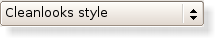
\includegraphics[scale=0.5]{graphics/combobox}
		}
		\subfigure[A Line Edit]{
			\label{lineeditfig}
			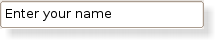
\includegraphics[scale=0.5]{graphics/lineedit}
		}
		\caption{Some of the various widgets used for editing data~\cite{QtGallery}}
		\label{editingWidgets}
	\end{figure}
  \begin{figure}
  \centering
  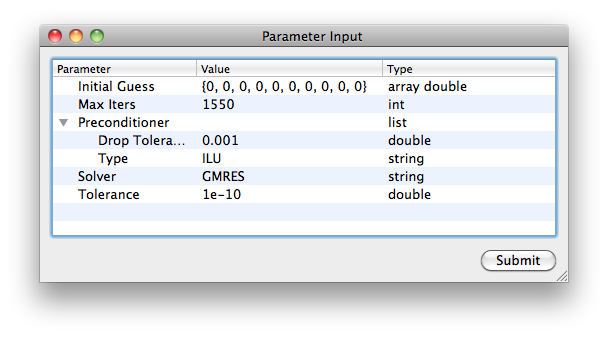
\includegraphics[scale=0.5]{graphics/basic_example}
  \caption[Basic GUI]{A basic Optika GUI}
  \label{basicexample}
  \end{figure} 
When all put together a basic Optika GUI looks something like Figure~\ref{basicexample}.
When the user clicks on a particular value, one of the above widgets pops up allowing them to edit the value.
Once the user is finished entering input, they click the action button (labled ``Submit'' in Figure~\ref{basicexample}).
The GUI then closes and the ParameterList used to help create the GUI now contains the input specified by the user.

\subsection{Underlying Technologies}
Optika is one of many packages in the Trilinos project~\cite{trilinos}, which is developed by Sandia National Labs. At it's core, 
the Trilinos project is a collection of various
libraries for aiding developers of scientific applications. Trilinos is best known for it's extensive colleciton of equation solvers,
but also provides a wealth of other tools that support general high performance computing. Each package in the Trilinos project provides
it's own set of unique capabilities. Optika is Trilnos's GUI package.

In order to provide GUI funcitonality, Optika relies on the Qt Framework~\cite{Qt}. 
Qt was choosen as Optika's backing GUI framework for several
reasons:
	\begin{itemize}
		\item It is cross-platform, allowing Optika to be used in many different computing environments.
		\item It is mature and has a comprehensive set of development tools. So we don't have to worry about major bugs.
		\item It has a rich feature-set, permiting Optika to grow in it's capbilities if necessary.
    \item It has a large user base.
		\item It has been used by Sandia in the past.
		\item The Optika lead developer was familiar with it.
	\end{itemize}
Because Trilinos is itself a library, relying on an additional third-party library can be a risky endevour. But
the qualities outlined above made using Qt a very easy choice. When choosing to use Qt we felt very confident that we 
would be able to rely on it to be stable, and to provide us with the tools we needed.

In order to configure and build Optika, the CMake~\cite{cmake} build system is used. This is the build system
used by Trilinos as a whole, so it makes perfect sense for Optika to use it as well. In addition, CMake
has support for the necessary special building tools required by Qt.

\section{Basic Optika Usage}
At the core of Optika is the ParameterList class from the Teuchos package~\cite{TeuchosPackage}, another part
of the Trilinos project. ParameterLists can be constructed either from within C++ source code or using XML.
In this paper, we will first start off with basic examples using C++ source code. However, once we start
talking about the more complex features we'll switch over to XML.
\subsection{Utilizing C++ to Create A GUI}
Since Tramonto is so sorely lacking in a quality user interface, we'll use it as an example of how to use Optika.
Let's look at the Dimenstion Control Parameters. These are just a few parameters used to define what kind of
dimensions are going to be used in the rest of the input file. Figure~\ref{basicTramonto} shows how we would create
such a GUI.
\begin{figure}
\centering
\lstinputlisting[language=C++]{basicTramonto/main.cpp}
\caption{Basic Tramonto Example}
\label{basicTramonto}
\end{figure}
We start by including the Optika\_GUI.hpp file. This include file allows us to use most of Optika's basic functionality.
Once in the main function we import several classes and functions into the namespace. We then create two
ParameterList RCPs~\cite{RCP}. Using the sublist function, the second 
ParameterList is defined as a sublist of the first. We provide them with the names ``Tramonto'' and
``Dimension Control Parameters''. The next several lines are calls to the set function. Each call
adds a Parameter to the ParameterList along with assigning it a default value and a documentation string (the 
documentation string is optional but highly encouraged). We then make
the all important call to the getInput function. This takes the list of parameters we have created and dynamically
generates a GUI which is then used to obtain input from the user. The end result is Figure~\ref{BasicTramontoScreenshot}.
\begin{figure}
\centering
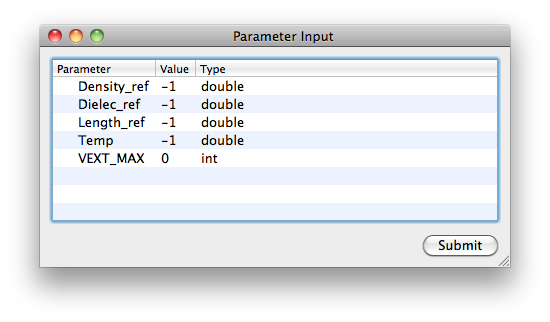
\includegraphics[scale=0.5]{graphics/BasicTramontoScreenshot}
\caption{The final product of the code in Figure~\ref{basicTramonto}}
\label{BasicTramontoScreenshot}
\end{figure}

\subsection{Utilizing XML to Create a GUI}
Using XML to declare your input parameters has a number of advantages over declaring you input in C++ source code.
\begin{itemize}
  \item XML is a lot cleaner than the corresponding C++. The source code approach can get pretty unruly, especially
  when some of the more advanced features of Optika are used.
  \item As an extension of being cleaner, using XML makes maintaining a user interface much simpler.
  \item When using XML, there is no need to recompile the entire program everytime a small change is made to the GUI.
\end{itemize}
If we redo the example we made in the previous section, but using XML, we end up with the C++ code and XML code found in
Figure~\ref{basicTramontoXML}. The XML code is rather strait forward. As in the C++ code we specify the name of the
parameter, it's default value, and a documentation string (the documentation xml attribute is optional, just like when using 
C++). When using XML we need to explicitly specify the type
of the parameter since this can't always be infered. Creating a ParameterList hierachy in XML is also arguable easier
in XML. ParameterLists just simply needed to be nested in one another.

Once the XML file describing the input parameters has been created, the GUI is created by using a slightly different
call to the getInput function. In this case the getInput function is pased the name of the XML file and an RCP pointing
to the ParameterList into which user input should be stored.
	\begin{figure}
		\subfigure[C++ Code]{
    \lstinputlisting[language=C++]{basicXMLTramonto/main.cpp}
		\label{basicXMLC++}
		}
		\subfigure[XML Code]{
     \lstinputlisting[language=XML]{basicXMLTramonto/inputs.xml}
		\label{basicXMLXML}
		}
		\caption{XML and C++ source code that can alternatively be used to create the GUI in Figure~\ref{BasicTramontoScreenshot}}
		\label{basicTramontoXML}
	\end{figure}

\section{Validators}
Often input parameters only have a certain set of valid values. Through the use of validators Optika allows application
developers to express these parameter constraints. When a validator is placed on a parameter, the generated GUI will
not allow the user to input invalid values for a parameter. Validators were also already part of the Teuchos package
before Optika was built, however the existing set of validators was sparse. Optika took the validator constructs that
were already in place and built on them, resulting in the construction of several new types of validators detailed below.
These new validators were then placed in the Teuchos package.

Validators are declared in a special section of the XML file. A special $<$Validators$>$ tag is declared as a direct child
of the root $<$ParameterList$>$ tag. In this $<$Validators$>$ tag all validators are declared. Each validator must specify at
least it's type and an ID using the $<$Validator$>$ tag. This ID can then be used anywhere in the rest of the XML file. 
To apply the validator to a parameter, simply add the validatorID xml attribute to the $<$Parameter$>$ tag. The same validator 
can be used on multiple parameters.

\subsection{Enhanced Number Validators}
Perhaps one of the most important validators is the Enhanced Number Validator. It allows the application developer
to specify minimum and maximum values for a numerical parameter. It also allows the developer to specify the
``step'' of a numerical parameter. The step of a numerical parameter is the amount by which the parameter's value
will be increased or decreased when the user clicks the up and down arrows on the spinbox being used to edit
the parameter's value. For non-integer numerical parameter's the Enhanced Number Validator also allows the
developer to declar with what precision the parameter's value should be displayed.

The XML Code in Figure~\ref{EnhancedNumberValidatorXML} shows an example of using an Enhanced Number Validator
to validate a parameter of type double. In the example we set the minimum acceptable value to be 0 and the 
maximum to be 10. The step is set to .5 so that the parameters value will change by .5 when the user clicks
up or down in the spinbox being used to edit the parameter. We also set the precision to two decimal places.
The validator is given the ID of 1 and applied thusly to the ``Double Parameter'' parameter using the validatorId
xml attribute. Notice how the type xml attribute of the validator is set to ``EnhancedNumberValidator(double)''. If we 
were validating a parameter of type into this xml attribute would be set to ``EnhancedNumberValidator(int)'', 
for a float it would be ``EnhancedNumberValidator(float)'', etc. These types must match up or an error will
occur.

With the exception of the validatorId xml attribute, all validator xml attribute demonstrated in Figure~\ref{EnhancedNumberValidatorXML}
are optional for an EnhancedNumberValidator. For example, you could only specify a minimum value of 0 to restrict all 
values of a parameter to positive values since no maximum was specified.
Appropriate defaults will be selected for step and precision if the developer chooses not to specify them.
\begin{figure}
\centering
\begin{lstlisting}[language=XML]
<ParameterList>
  <Parameter name="Double Parameter" value="1.0" type="double" 
    docString="A double parameter" validatorId="1" />
    ...Other Parameters ....
  <Validators>
    <Validator type="EnhancedNumberValidator(double)" 
      min="0" max="10" step=".5" precision="2" validatorId="1"/>
  </Validators>
</ParameterList>
\end{lstlisting}
\caption{Example Usage of an Enhanced Number Validator}
\label{EnhancedNumberValidatorXML}
\end{figure}

\subsection{String Validators}
String Validators are a simple yet powerful tool to restrict string input. String input can be a nice alternative to
using some standard set of integer values to represent various settings for a parameter. The problem is a simple wrong 
keystroke can cause big problems. By using a String Validator an application developer can ensure that a user 
only selects a string value that is appropriate for a given parameter. 
String Validators may only be used on parameters of stype std::string, otherwise an error will occur.
\begin{figure}
\centering
\begin{lstlisting}[language=XML]
<ParameterList>
  <Parameter name="String Parameter" value="Option 1" type="string" 
    docString="A string parameter" validatorId="1" />
    ...Other Parameters ....
  <Validators>
    <Validator type="StringValidator" validatorId="1">
      <String value="Option 1"/> 
      <String value="Option 2"/> 
      <String value="Option 3"/> 
    </Validator>
  </Validators>
</ParameterList>
\end{lstlisting}
\caption{Example Usage of an String Validator}
\label{StringValidatorXML}
\end{figure}
Figure~\ref{StringValidatorXML} shows how to use a String Validator. Children $<$String$>$ tags with a manditory ``value'' xml attribute specify which values are valid.
In this example ``Option 1'', ``Option 2'', and ``Option 3'' will be the only values the user can select from the GUI.

\subsection{Filename Validators}
Filename Validators allow application developers to designate a string parameter as a filename. When applied to a parameter,
any attempt to edit that parameter will result in the user being presented with a special file selector widget (Figure~\ref{fileSelectorWidget}). If the 
``fileMustExist'' xml attribute is set to true, the the user will only be able select files that already exist. Otherwise, the user will be able
to select any file he/she wants. Filename Validators can only be applied to parameters of type string. \begin{figure}
\centering
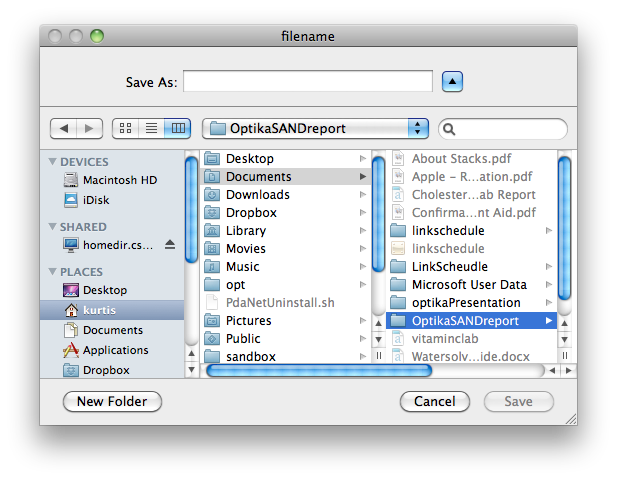
\includegraphics[scale=0.5]{graphics/fileWidget}
\caption{The file selector widget presented to the user when a Filename Validator is applied to a parameter}
\label{fileSelectorWidget}
\end{figure}
\begin{figure}
\centering
\begin{lstlisting}[language=XML]
<ParameterList>
  <Parameter name="Output File Name" value="" type="string" 
    docString="Name of the output file." validatorId="1" />
    ...Other Parameters ....
  <Validators>
    <Validator type="FilenameValidator" fileMustExist="false" 
      validatorId="1">
  </Validators>
</ParameterList>
\end{lstlisting}
\caption{Example Usage of an Filename Validator}
\label{filenamevalidatorXML}
\end{figure}
Figure~\ref{filenamevalidatorXML} shows an example of how to use a Filename Validator. Here we use it to select a file to output the results
of our program. We set the ``fileMustExist'' xml attribute to false so that the user can select a file that doesn't already exist.

\subsection{Array Validators}
Array Validators allow any of the above described Validators to be used on a array parameter. For example, we might want to use a
String Validator on an array of strings. To do with we'd create and Array Validator with a ``prototype'' String Validator. The 
``prototype'' validator is just a term used to describe the validator the developer would like to be applied to each entry of an
array. Prototype validators can be specified in one of two ways. First, the developer can code the validator as child of the array validator
tag as in Figure~\ref{actualArrayValidatorXML}. In this case, the prototype validator does not need an ID. 
Second, the developer can simply specify another validator as array validator's  prototype by using the
``prototypeId'' xml attribute as in Figure~\ref{protoAttributeArrayXML}. This second option allows you to reuse the prototype validator in other instances.

When creating an ArrayValidator, the type xml attribute will include both the type of the prototype validator and the type of the array
parameter. For instance, if we were using a prototype Filename Validator on a string parameter, the value of our type xml attribute would
be ``ArrayValidator(FilenameValidator, string)''. It is crucial that all of these types match up otherwise errors will occur.

\begin{figure}
\centering
\begin{lstlisting}[language=XML]
<ParameterList>
  <Parameter name="Options" value="{Option 1, Option 1, Option 1}" 
    type="Array(string)" docString="An array of options" 
    validatorId="1" />
    ...Other Parameters ....
  <Validators>
    <Validator type="ArrayValidator(StringValidator, string)" 
      validatorId="1">
      <Validator type="StringValidator">
        <String value="Option 1"/>
        <String value="Option 2"/>
        <String value="Option 3"/>
      </Validator>
    </Validator>
  </Validators>
</ParameterList>
\end{lstlisting}
\caption{Example Usage of an Array Validator in which the prototype is declared as a child of the array validator.}
\label{actualArrayValidatorXML}
\end{figure}
\begin{figure}
\centering
\begin{lstlisting}[language=XML]
<ParameterList>
  <Parameter name="Output File Name" value="{Option 1, Option 1}" 
    type="Array(string)" 
    docString="Name of output file." validatorId="1" />
    ...Other Parameters ....
  <Validators>
    <Validator type="ArrayValidator(StringValidator, string)" 
      validatorId="1" prototypeId="2"/>
    <Validator type="StringValidator" validatorId="2">
      <String value="Option 1"/>
      <String value="Option 2"/>
      <String value="Option 3"/>
    </Validator>
  </Validators>
</ParameterList>
\end{lstlisting}
\caption{Example Usage of an Array Validator in which the prototype is specified using the prototypeId xml attribute.}
\label{protoAttributeArrayXML}
\end{figure}

\section{Dependencies}
Dependencies are the crown jewel of Optika. They allow application developers to express common dependenices that occur between
parameters in their program. At their core dependencies allow a developer to say ``based on the state of parameter A, parameter be should
behave in a certain way.'' In this case, we would say parameter A is the ``dependee'' parameter and parameter B is the ``dependent'' parameter.
All dependencies have at least one dependee and one dependent. When running the GUI, the algorithm for expressing dependencies is as follows:
\begin{enumerate}
	\item A parameter's value is changed by the end-user.
	\item The GUI queries the associated defined dependencies to see whether or not the parameter that changed has any dependents.
	\item If the parameter does have dependents, the GUI requests a list of all the dependencies in which the changed
	parameter is a dependee.
	\item For each dependency, the evaluate function is called. The dependency makes any necessary changes to the dependent parameter
	and the GUI updates with the new data.
	\item If any dependents now have invalid values, focus is given to them and the end-user is requested to change their value to
	something more appropriate.
\end{enumerate}
Like validators, dependencies are declared in the XML using the $<$Dependencies$>$ tag that must be a direct child
of the root $<$ParameterList$>$ tag. Inside the $<$Dependencies$>$ tag each dependency is declared using the $<$Dependency$>$ tag. Within the
$<$Dependency$>$ tag the xml attribute ``type'' is required in order to define the type of the dependency. Each $<$Dependency$>$ must have at least
one $<$Dependee$>$ child tag and one $<$Dependent$>$ child tag. Each of these tags must have an xml attribute called ``parameterId'' which identifies
their associated parameter.

\subsection{Visual Dependencies}
Visual dependencies allow the application developer to show and hide parameters based on other paramters' values. This is useful in situations where
when a parameter takes on a particular value, another parameter is no longer relevant. By hiding this now irrelevant parameter from the user the
application developer can hopefully avoid some confusion. If we were to write these dependencies as a sentance they would say: ``Based on
the value of the dependee parameter show or hide the dependent parameter(s)''.

Visual dependencies have an extra boolean xml attribute that can be put in the $<$Dependency$>$ tag called ``showIf''. What ever dependee is being tested to 
determine the dependents visibility, showIf can negate it by being set to false. So if a visual dependency is set to only show a dependent when the
dependee has a parituclar value, setting showIf to false will cause the dependent to be visible only when the dependee \emph{does not} have a particular
value. If the showIf attribute is not present, it is assumed to be true. All visual dependencies may have an aribitray number of dependents of any type.
Dependents can also be parameter lists.

\subsubsection{String Visual Dependencies}
String Visual Dependencies allow an application developer to base whether or not a parameter is visible on the particular string value of another
parameter. For instance, we might say if parameter A is equal to the value ``Swiss Cheese'' or ``Cheedar Cheese''the show parameter B. Otherwise, do not 
show parameter B. Figure~\ref{StringVisXML} demonstrates how we would express this in XML.  If in figure~\ref{StringVisXML} we set the showIf xml attribute to false then the ``How much do you like that cheese?'' parameter will only be showed when ``Favorite Food'' \emph{does not} equal ``Swiss'' or ``Cheddar''.
String Visual dependencies must have a single dependee of type string. 
\begin{figure}
\centering
\begin{lstlisting}[language=XML]
<ParameterList>
  <Parameter name="Favorite Food" type="string" value="pasta"
    id="1" docString="Your favorite food."/>
  <Parameter name="Rate the cheese please" type="int" value="5"
    docString="A rating of cheese" id="2"
    ...Other Parameters ....
  <Dependencies>

    <Dependency showIf="true" type="StringVisualDependency">
      <Dependee parameterId="1"/>
      <Dependent parameterId="2"/>
      <StringValues>
        <String value="Swiss"/>
        <String value="Cheddar"/>
      </StringValues>
    </Dependency>

  </Dependencies>
</ParameterList>
        
\end{lstlisting}
\caption{Example Usage of a String Visual Dependency.}
\label{StringVisXML}
\end{figure}

\subsubsection{Bool Visual Dependencies}
Bool Visual Dependencies allow the developer to base the visibility of a parameter on the boolean value of another parameter. For instance, we might say
if parameter A is set to true then we want to show parameter list B. Figure~\ref{BoolVisXML} shows how a developer would implement this in XML. If the
showIf xml attribute were set to false then the ``Special Parameters'' parameter list would only be shown when ``Use special parameters'' was set to false.
Bool Visual Dependencies must have a single depenedee of type bool.
\begin{figure}
\centering
\begin{lstlisting}[language=XML]
<ParameterList>
  <Parameter name="Use special parameters" type="bool" value="true"
    id="1" docString="Whether or not to use special parameters"/>
  <ParameterList name="Special Parmeters" type="int" id="2"
    docString="special parameters only used in certain instances" 
    ...Special Parameters ....
  </ParameterList>
  <Dependencies>

    <Dependency showIf="true" type="BoolVisualDependency">
      <Dependee parameterId="1"/>
      <Dependent parameterId="2"/>
    </Dependency>

  </Dependencies>
</ParameterList>
\end{lstlisting}
\caption{Example usage of a Bool Visual Dependency}
\label{BoolVisXML}
\end{figure}

\subsubsection{Number Visual Dependencies}
Number Visual Dependencies allow the developer to base the visibility of a parmeter on the numerical value of another parameter. In their simpliest form
Number Visual Dependencies simply check to see if the dependees value is greater then or equal to zero. If the value is greater than or equals to zero the
dependent(s) will be shown. Otherwise, the dependents will be hidden. If the showIf xml attribute value is set to false, then the visibility results will
be the opposite. Figure~\ref{NumberVisXML1} shows basic usage of a number visual dependency. Unless the ``Temperature'' parameter is below zero degrees
celsius then we can't have any ice cubes in the room. We do this by setting the showIf xml attribute to false so that ``Number of ice cubes'' only shows
when the ``Temperature'' parameter is below zero.
\begin{figure}
\centering
\begin{lstlisting}[language=XML]
<ParameterList>
  <Parameter name="Temperature" type="double" value="1" id="1" 
    docString="The temperature in the room in degrees celsius"/>
  <Parameter name="Number of ice cubes" type="int" value="1"
    id="2" docString="The number of ice cubes in the room"/>
  <Dependencies>

    <Dependency 
      showIf="false" 
      type="NumberVisualDependency(double)"
    >
      <Dependee parameterId="1"/>
      <Dependent parameterId="2"/>
    </Dependency>

  </Dependencies>
</ParameterList>
  \end{lstlisting}
  \caption{Example usage of a Number Visual Dependency.}
  \label{NumberVisXML1}
\end{figure}
Notice in figure~\ref{NumberVisXML1} that like Enhanced Number Validators, the type value of a Number Visual Dependency has to include the type of the
parameter it's evaluating (in this case a double). Number visual dependencies may have only one dependee. The type of that dependee must match up with the
type specified in the type xml attribute used in the Number Visual Dependency tag.

Sometimes it is necessary to test a number typed parameter using criteria other than whether or not it's current value is greater than or equal to zero.
This can be accomplished by using a $<$Function$>$ tag. A $<$Function$>$ tag instructs the dependency to run the value of the dependee through a funciton
first, and then test the result of that function to see if it is greater than or equal to zero. Consider the example in figure~\ref{NumberVisXML1}, only this
time let's say our temperature is in degrees farenheit. In order to get the proper functionality, we'll add a ``subtraction function'' to the dependency that will
subtract 32 from the value of the temperature parameter before it is tested against zero. Figure~\ref{NumberVisXML2} shows an example of this. We set the operand 
xml attribute to 32 and the type of the function to ``SubtrationFunction(double)''\footnote{For a complete list of available funcitons see Appendix~\ref{sec:funcs}}
 since we want to use a subtraction function on a parameter of type double.
\begin{figure}
\centering
\begin{lstlisting}[language=XML]
<ParameterList>
  <Parameter name="Temperature" type="double" value="33" id="1" 
    docString="The temperature in the room in degrees farenheit"/>
  <Parameter name="Number of ice cubes" type="int" value="1"
    id="2" docString="The number of ice cubes in the room"/>
  <Dependencies>

    <Dependency 
      showIf="false" 
      type="NumberVisualDependency(double)"
    >
      <Dependee parameterId="1"/>
      <Dependent parameterId="2"/>
      <Function operand="32" type="SubtractionFunction(double)"/> 
    </Dependency>

  </Dependencies>
</ParameterList>
\end{lstlisting}
\caption{Example usage of a Number Visual Dependency using a function.}
\label{NumberVisXML2}
\end{figure}

\subsection{Validator Dependencies}
A Validator Dependency is a dependency in which the validator that is in use on the dependee is dependent upon the value of the dependee. Both the type of
the dependee and the dependent will vary with each type of validator dependency and parameter type of the dependent. Validator Dependencies will always have
one dependee. Also, dependent parameters in a Validator Dependency will never be a parameter list. A validator dependency can have an arbitrary number of 
dependents.

\subsubsection{String Validator Dependency}
A String Validator Dependency allows the application developer to change the validator used on a dependent based on the string value of the dependee
parameter. This is accomplished by mapping values the dependee might take on to corresponding validators. Also, a default validator may be specified.
This way, if the dependee takes on a value that has not been mapped to a validator the default validator can be used. 

A String Validator Dependency must comply with the following rules:
\begin{itemize}
\item The dependee must be of type string
\item All of the validators which have values mapped to them must be of the same type.
\item If specified, the default validator must be of the same type of validator used in the map.
\item The validators in the map and the default validator should be appropriate for the parameter type of the dependent(s).
\end{itemize}

Figure~\ref{StringValiDepXML} shows an example of how to use a String Validator Dependency. In this example we have two parameters, ``Temperature Scale''
and ``Freezer Temperature''. If ``Temperature Scale'' is set to Farenheit we want to restrict the values on ``Freezer Temperature'' to 0 through 50. But
if ``Temperature Scale'' is set to Celsius, we want to use a validator with the corresponding celsius values for 0 and 50. If the user enters something else
for ``Temperature Scale'' we'll just default to using the Farenheit validator.  Note that we could improve this example by putting a string validator on 
the temperature scale parameter, restricting it's values to Celsius and Farenheit.  This would effectively eliminate the need for us to specify a default 
validator.
\begin{figure}
  \centering
\begin{lstlisting}[language=XML]
<ParameterList>
  <Parameter name="Temperature Scale" type="string" value="Celsius"
    id="1" docString="The temperature scale being used"/>
  <Parameter name="Freezer Temperature" type="double" value="0"
    id="2" docString="The temperature in the freezer"/>
  <Validators>
    <Validator type="EnhancedNumberValidator(double) validatorId="1"
      min="0" max="50"/>
    <Validator type="EnhancedNumberValidator(double) validatorId="2"
      min="-17.77" max="10"/>
  <Validators>
  <Dependencies>
    <Dependency 
      type="StringValidatorDependency" 
      defaultValidatorId="2"
    >
      <Dependee parameterId="1"/>
      <Dependent parameterId="2"/>
      <ValuesAndValidators>
        <Pair value="Farenheit" validatorId="1"/>
        <Pair value="Celsius" validatorId="2"/>
      </ValuesAndValidators>
    </Dependency>
  </Dependencies>
</ParameterList>
\end{lstlisting}
\caption{Example usage of a String Validator Dependency.}
\label{StringValiDepXML}
\end{figure}

\subsubsection{Range Validator Dependency}
Range Validator Dependencies work very similarliy to String Validator Dependencies in that they map validators to specific dependee values. However,
instead of mapping string values to validators, Range Validator Dependencies map ranges of numbers to validators. If the dependee's value falls within one of the 
mapped ranges, then that range's associated validator is applied to the dependent(s). A range is specified by defining it's minimum (inclusive) and it's maximum (exclusive).
Also like String Validator Dependencies, a default validator can be specified. If the dependees value does not fall with in one of the mapped ranges the default validator is 
then used. A Range Validator Dependency must conform to the following constraints:
\begin{itemize}
\item The dependee must be a number type.
\item All of the validators used specified in the mapping must be of the same type.
\item If specified, the default validator must be of the same type as the validators specified in the map.
\item The validators specified in the map must be appropriate for the type of the dependent(s).
\end{itemize}

Figure~\ref{RangeValiDepXML} shows and example of a Range Validator Dependency. In it, we want to use different validators
on the ``Fondue Food'' if the Fondue Pot Temperature is different. If the temperature is greater than or equal to 80 or less than 120,
we only want the user to be able to select ``Cheese'' or ``Bread''. If it's greater than or equal to 120 but less than 180, we only want the
user to be able to pick ``Chicken'' or ``Beef''. We associated these ranges with their appropriate values in the $<$RangesAndValidators$>$ by
using $<$Pair$>$ tags for each range and validator. Notice that like Enhanced Number Validators and Number Visual Dependencies, the type of the dependee parameter is 
included in the type xml attribute of the dependency. In Figure~\ref{RangeValiDepXML} the dependee's type is double so the type of the dependency is 
``RangeValidatorDependency(double)''.
\begin{figure}
  \centering
\begin{lstlisting}[language=XML]
<ParameterList>
  <Parameter name="Fondue Pot Temperature" type="int" value="100"
    id="1" docString="The number of dimensions being used"/>
  <Parameter name="Fondue Food" type="string" value="Cheese"
    id="2" docString="The surface type"/>
  <Validators>
    <Validator type="StringValidator" validatorId="1">
      <String value="Cheese"/>
      <String value="Bread"/>
    </Validator>
    <Validator type="StringValidator" validatorId="2">
      <String value="Chicken"/>
      <String value="Beef"/>
    </Validator>
  <Validators>
  <Dependencies>
    <Dependency type="RangeValidatorDependency(double)">
      <Dependee parameterId="1"/>
      <Dependent parameterId="2"/>
      <RangesAndValidators>
        <Pair min="80" max="120" validatorId="1"/>
        <Pair min="120" max="180" validatorId="2"/>
      </ValuesAndValidators>
    </Dependency>
  </Dependencies>
</ParameterList>
\end{lstlisting}
\caption{Example usage of a Range Validator Dependency.}
\label{RangeValiDepXML}
\end{figure}
 

\subsubsection{Bool Validator Dependency}
A Bool Validator Dependency allows the developer to apply one validator to the dependent(s) when the dependee is true, and another validator
to the dependent(s) when the dependee is false. You could also specify one validator to be applied when the dependee is true and no validator
to be applied when the dependee is false (or vice versa). The dependee of a Bool Validator Dependency must be of type bool. If both a ``true'' and
``false'' validator are specified, they must be of the same type. Also, the validator(s) specified must be appropriate for the dependent(s).

Figure~\ref{BoolValidDepXML} shows an example of a Bool Validator Dependency. In this example we only want a validator to be placed on the
``Temperature'' parameter if ``Has Temperature Constraints'' is set to true. Therefore we set the trueValidatorId xml attribute to the id of the
validator we want to use and don't specify a validator to be used if the dependee is false.
\begin{figure}
\centering
\begin{lstlisting}[language=XML]
<ParameterList>
  <Parameter name="Has Temperature Constraints?" type="bool" 
    value="true" id="1" 
    docString="Whether or not temperature constratins should be used."/>
  <Parameter name=" Temperature" type="double" value="0"
    id="2" docString="The temperature"/>
  <Validators>
    <Validator type="EnhancedNumberValidator(double) validatorId="1"
      min="0" max="50"/>
  <Validators>
  <Dependencies>
    <Dependency 
      type="BoolValidatorDependency" 
      trueValidatorId="1"
    >
      <Dependee parameterId="1"/>
      <Dependent parameterId="2"/>
    </Dependency>
  </Dependencies>
</ParameterList>
\end{lstlisting}
\caption{Example usage of a Bool Validator Dependency.}
\label{BoolValidDepXML}
\end{figure}

\subsection{Number Array Length Dependencies}
Number Array Length Dependencies allow the application developer to have the length of an array parameter determined by the value of another parameter. Number Array Length
Dependencies must have a dependee with an integer type and the dependent(s) must be an array. Unless otherwise specified, the value of the dependee parameter is directly
used for the length of the dependent array parameter(s). 

Figure~\ref{ArrayLengthXML} shows an example of an Number Array Length Dependency. When the ``Number of buckets'' parameter changes, the array in the ``Amount
in each bucket'' shrinks and expands accordingly. Note how in the type xml attribute for the dependency we had to specify both the type of the dependee and the
dependent. Are you starting to notice a theme?
\begin{figure}
\centering
\begin{lstlisting}[language=XML]
<ParameterList>
  <Parameter name="Number of buckets" type="int"
    value="2" id="1" 
    docString="The number of buckets we have."/>
  <Parameter name="Amount in each bucket" 
    type="array(double)" value="{0,0}"
    id="2" docString="The amount of water in each bucket"/>
  <Dependencies>
    <Dependency type="NumberArrayLengthDependency(int, double)">
      <Dependee parameterId="1"/>
      <Dependent parameterId="2"/>
    </Dependency>
  </Dependencies>
</ParameterList>
\end{lstlisting}
\caption{Example usage of a Bool Validator Dependency.}
\label{BoolValidDepXML}
\end{figure}

If we wanted the length of the array to be based on something other then the direct value of the dependee parameter, we could run it through a function. This would 
be done by adding a $<$Function$>$ tag inside the $<$Dependency$>$ tag, just like we did in figure~\ref{NumberVisXML2} for the Number Visual Dependency.

\section{Condition Visual Dependency}
Up until this point, all the dependency have had only a single dependee. A Condition Visual Dependency is a special Visual Dependency that allows you to base the visibility
of the dependent parameter(s) upon the state of multiple dependees. This is accomplished via the use of Conditions.
\subsection{Parameter Conditions}

\subsubsection{String Condition}

\subsubsection{Number Condition}

\subsubsection{Bool Condition}

\subsection{Binary Logic Conditions}

\subsubsection{And Condition}

\subsubsection{Or Condition}

\subsubsection{Equal Condition}

\subsection{Not Condition}

\subsection{Using A Condition Visual Dependency}



\section{Other Features of Optika}
\subsection{Custom Functions}
In additition to the traditional work flow of just calling the getInput function, Optika also allows for the specification of ``custom functions.''

\subsection{Customizing Look And Feel}
There are a number ways


\section{Future Developement}

\section{Contributions}
